\section{Congruence Closure}

This problem is a generalization of the previous problem
including first-order formulas (constant and functional symbols)
and equality between terms. Let $TERMS(H)$ be the set of terms in the Horn
formula $H$. Special attention is given to functional symbols, which they
are uninterpreted. Equations are handled using the UNION-FIND
data structure. If there exist In \cite{GALLIER1987233}, the author
introduces to graphs to represent information about the
Horn formula. The first graph is the graph of subterm dependencies
$GT(H)$ in the Horn formula $H$, where all subterms form the vertices of the graph and
a directed edges from node $x$ to $y$ is $y$ is a subformula of
$x$.

\begin{figure}[h]
  \centering
  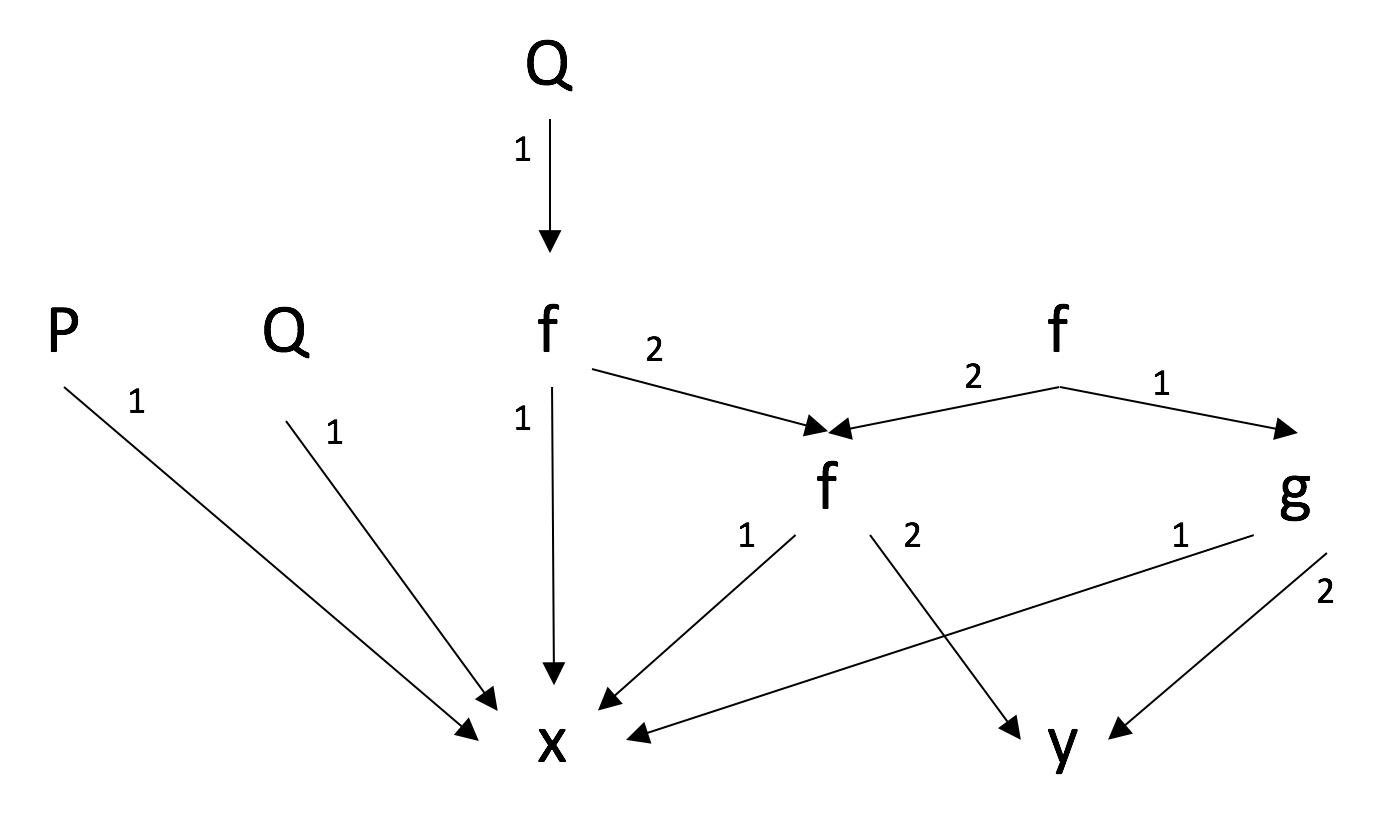
\includegraphics[width=8cm]{GT1}
  \caption{Graph of subterm dependencies for the Horn formula $P(x) :- f(g(x, y), f(x, y)) = y, x = f(x, y) \land Q(f(x, f(x, y))) \land :- Q(x)$}
\end{figure}

The second graph $GC(H)$ encodes the relation between the terms
in the Horn formula $H$, i.e. the vertices are the equations (a predicate $P$
can be `transformed' into an equation of the form $P = \top$)
present in the $H$ (which doesn't include all subterms necessarily), and
there is a directed edge between vertices $x$ and $y$ with label $C$
if there exists a Horn clause $C$ such that $x = head(C)$ and $y \in body(C)$.
The reason for the direction of the edges in $GC(H)$ is because for each node $x$ in
this graph we can check their `successors' with label $C$ (technically the
atomic formulas in the body of the Horn clause $C$) and decide if we should merge
the elements in the equation of $x$ using the UNION-FIND data structure.

\begin{figure}[h]
  \centering
  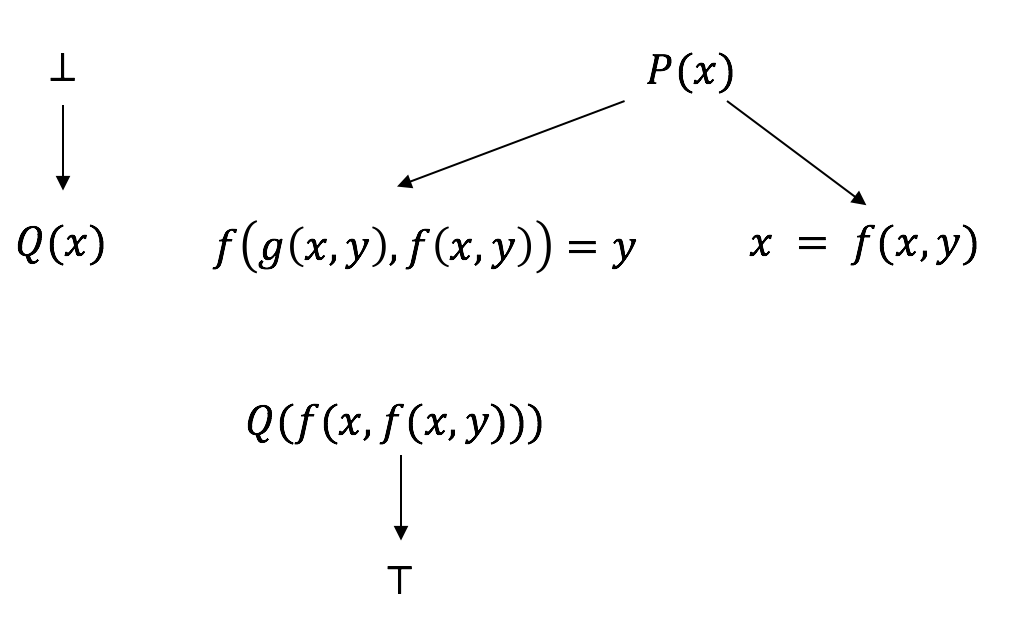
\includegraphics[width=8cm]{GC1}
  \caption{Graph of equations in the Horn formula $P(x) :- f(g(x, y), f(x, y)) = y, x = f(x, y) \land Q(f(x, f(x, y))) \land :- Q(x)$}
\end{figure}

It is important to mention that the author in \cite{GALLIER1987233} generalizes
the concept of equality to describe different types, i.e. we can have more than
one equality between terms. Nonetheless, for the purpose of our work only
one equality is needed between terms. For the latter, some modifications
to the definitions are done in order to keep consistency with our goals.

Also, the author distinguishes two types of closures: in order to compute
the congruence closure of a set of ground Horn clauses implicational and
equational. The implicational closure is essentially the same as described
before in the previous section with the minor change of extending the propositional
formulas to free first-order formulas with equalities. A formal definition of
the equational closure is given as follows:

\definition{\cite{GALLIER1987233}} Let $GT(H)$ be a graph of subterm dependencies for
a given grounded Horn formula $H$ with equalities. An \textit{equational congruence} on $GT(H)$
is a family $R$ of relations $R_i$ (partitions) over $TERMS(H)$ iff:

\begin{itemize}
\item Each $R_i$ is an equivalence relation.
\item For every pair (u, v) in $TERMS(H) \times TERMS(H)$, if the functional names
  of the terms $u, v$ are the same (i.e. they are either both constants or both functions with same name),
  $u \in R_i$, and for each argument of $u$ and $v$ they belong to some relation $R_j$ then $uR_iv$. 
\end{itemize}

The combination of both implicational and equational closure leads to the
congruence closure of a given theory. In fact, the author proved in \cite{GALLIER1987233}
the existance of such closure by interleaving both implicational and equational closure.
Nonetheless, extracting an algorithm from the constructive proof mentioned above
would lead to an inefficient algorithm for computing the congruence closure. Instead, the
author systematically combines a similar approach of implicational closure as we studied
before on the previous section and adding the equational closure component by merging
terms using the UNION-FIND data structure. It is not hard to see that implicational closure
can produce more equations to be merged and the equational closure can lead to new equations
to be satisfiable in the body for Horn clauses. Nonetheless, since there is a finite
number of atomic formulae (equations) and a finite number of Horn clauses, then by interleaving
both closures we can guarantee termination.

The algorithm mentioned in \cite{GALLIER1987233} is an extended version of the algorithm in
\cite{DOWLING1984267} including an \textit{equational congruence} algorithm that checks for
the equational closure mentioned above and the data structure UNION-FIND to deal with equations.
There are two versions of this algorithm. The first one uses a procedure to compute the equational
congruence checking the sucessor for the terms involved each time. As a result, the running time
of the algorithm is $\bigO{m n}$, where $m$ is the number of Horn clauses and $n$ is the number
of atomic formuale. A second refinement utilizes the fast congruence closure algorithm
\cite{Downey:1980:VCS:322217.322228} which obtains a $\bigO{n \log n}$ running time. In order
to become an efficient implementation, several data structures are considered. For each equation
in the Horn formula, we add two records containing the representative element of the left hand side
term and the right hand side term respectively. When merging terms into an equivalence class, it
is considered as the representative the element which has more terms in the tree representation
of the respective equivalence class, hence a `modify the smaller half' heuristic is achieved. This
last heuristic plays an important role to obtain the running time of the algorithm. 

As a side comment, the literature is inconsistent at this point in the sense
that different authors use the same name to describe different problems. In the latter, the term
congruence closure refers to a similar notion of equational closure as studied before in the
previous section.

A `signature' for a functional symbol of the form $f(x_1, \dots, x_n)$ with $n \geq 1$, 
in the sense of \cite{Downey:1980:VCS:322217.322228}, corresponds to the $n-tuple$
$(\alpha(1), \dots, \alpha(n))$, where the function $\alpha : TERMS(H) \rightarrow \mathbb{N}$
is a mapping from the set of terms in the Horn formula to a natural number that encodes
the respective partition in the family of relations $R$. 
The fast congruence closure algorithm described in 
\cite{Downey:1980:VCS:322217.322228} considers two terms to be
`congruent' is their `signatures' are the same. Contrary to the notion of signature in
\cite{GALLIER1987233}, the signtare does no include the name of the respectively terms.
Nonetheless, we can always include functional symbol name as one of the arguments
in the functional symbol signature.

The key addition of the fast congruence closure algorithm is the `Signature Table'. Together
with a UNION-FIND data structure updates only the elements and their signatures as needed,
whereas the previous algorithm updates all terms signatures all the time, even when
they might not be used in the future. Let us describe the operations of these data structures:

UNION-FIND operations:
\begin{itemize}
\item \textit{find(v)}: Given a vertex $v$ in $GT(H)$, return the name of the equivalence
  class containing $v$.
\item \textit{list(e)}: Given a representation $e$ for some equivalence class, return
  the list of vertices with at least one succesor in $e$, i.e. return the set of
  predecessors for all vertices $v$ such that $v \in e$.
\item \textit{union($e_1, e_2$)}: Given two disjoint equivalent classes $e_1, e_2$, combine
  $e_1, e_2$ into a single equivalence class with $e_1$ as representative.
\end{itemize}

SIGNATURE-TABLE operations:
\begin{itemize}
\item \textit{enter(v)}: Given a vertex $v$ from $GT(H)$, store $v$ in the signature
  table with its current signature.
\item \textit{delete(v)}: Given a vertex $v$ from $GT(H)$, delete $v$ from the
  signature table if it is present.
\item \textit{query(v)}: Given a vertex $v$ from $GT(H)$, if there exists a vertex $w$ in
  $GT(H)$ stored in the signature table with same signature as $v$, then return $w$; otherwise
  return $\Lambda$.
\end{itemize}

Two additional sets are needed to keep track of the changes made by the algorithm. The set
\textit{pending} which is a list of vertices to be entered in the signature table, typically
this set is updated when elements are being merged in the UNION-FIND data structure
(equational closure); and \textit{combine}, which is a list of pairs of vertices whose
equivalence classes are to be combined, this structure is updated after performing implicational
closure on the current set of terms and signatures. The fast congruence closure algorithm
is shown in \textbf{Algorithm 1}.

\label{fastCongruenceClosureAlg}
\begin{algorithm}[h]
  $pending = \{v \in V_1 \vert d(v) \geq 1\}$\;
  \While{$pending \neq \empty$}{
    $combine = \emptyset$\;
    \For{each v $\in$ pending}{
      \eIf{$query(v) = \Lambda$}{
        enter(v)\;
      }{
        add (v, query(v)) to combine\;
      }
    }
    $pending = \emptyset$\;
    \For{each (v, w) $\in$ combine}{
      \If{$find(v) \neq find(w)$}{
        \eIf{$|list(find(v))| < |list(find(w))|$}{
          \For{each u $\in$ list(find(v))}{
            delete(u)\;
            add u to pending\;
          }
          union(find(w), find(v))\;
        }{
          \For{each u $\in$ list(find(w))}{
            delete(u)\;
            add u to pending\;
          }
          union(find(v), find(w))
        }
      }
    }
  }
  \caption{The fast congruence closure algorithm}
\end{algorithm}

One invariant of this algorithm is that the signature table
stores vertices in such a way that a signature is never repeated.
This fact comes from observing the for loop at lines 4 - 10. In fact,
any vertex stored at the signature table is the has the most updated
signature and its the reprensetative of the equivalence class.

Regarding implementation details, it is important to mention that the authors
perform a linear transformation on $GT(H)$ such that any functional symbol
contains at most two successors. This is done by a `currying' the formula,
i.e. for any functional symbol $x$ with 1 or 2 successors return the same
vertex representation; otherwise, if the number of successors of $x$ is $n$
with $n > 2$, then introduce a new functional symbol and recursively solve
for the last $n - 1$ arguments of $x$, let us call $x^{'}$ this new functional
symbol, then make an edge between $x$ and its first argument of $x$ and $x^{'}$.

After applying this currying process, all terms will contain at most two
arguments/successors. Because of that, the signature table only requires to
deal with two parts, with the terms with one successor and terms with two
successors. The first part can easily achieve $\bigO{1}$ running time in
all the operations using an array. For the second part, the authors propose
several implementation with different data structures like balanced binary trees,
hash tables, arrays of arrays, etc. Naturally, different running times are
achieved in both running time and space complexity.

To illustrate the algorithm, an example by hand is shown below applying the fast
congruence closure to the equivalence classes $C_0 = \{ \{a, b, f^3 a, f^5 a\}_1 ,\{f a\}_2 ,\{f b\}_3 ,\{f^2 a\}_4 ,\{f^4 a\}_5\}$:

\begin{itemize}
  \item $C_0 = \{ \{a, b, f^3 a, f^5 a\}_1 ,\{f a\}_2 ,\{f b\}_3 ,\{f^2 a\}_4 ,\{f^4 a\}_5\}$
  \item $pending = \{f a, f b, f^2 a, f^3 a, f^4 a, f^5 a\}$
  \item $list(1) = \{f a, f b, f^4 a\}$; $list(2) = \{f^2 a\}$; $list(3) = \{\}$; $list(4) = \{f^3 a\}$; $list(5) = \{f^ 5 a\}$
  \item $combine = \{\}$
  \item $sig\_table = \{(f a, (1))\}$
  \item $combine = \{(f a, f b)\}$
  \item $sig\_table = \{(f a , (1)), (f^2 a , (2) )\}$
  \item $sig\_table = \{(f a , (1)), (f^2 a , (2) ), (f^3 a, (4))\}$
  \item $combine = \{(fa, fb), (fa, f^4 a)\}$
  \item $sig\_table = \{(f a , (1)), (f^2 a , (2) ), (f^3 a, (4)), (f^5 a, (5))\}$
  \item $pending = \{\}$
  \item $C_1 = \{\{a, b, f^3 a, f^5 a\}_1 ,\{f a, f b\}_2  ,\{f^2 a\}_4 ,\{f^4 a\}_5\}$
  \item $sig\_table = \{(f a , (1)), (f^2 a , (2) ), (f^3 a, (4))\}$
  \item $pending = \{f^5 a\}$
  \item $C_2 = \{\{a, b, f^3 a, f^5 a\}_1 ,\{f a, f b, f^4 a\}_2  ,\{f^2 a\}_4 \}$
  \item $list(1) = \{f a, f b, f^4 a\}$; $list(2) = \{f^2 a, f^5 a\}$; $list(3) = \{\}$; $list(4) = \{f^3 a\}$; $list(5) = \{\}$
  \item $combine = \{\}$
  \item $combine = \{(f^2 a, f^5 a)\}$
  \item $pending = \{\}$
  \item $sig\_table = \{(fa, (1)), (f^2 a, (2))\}$
  \item $pending = \{f ^ 3 a\}$
  \item $C_3 = \{\{a, b, f^3 a, f^5 a, f^2 a\}_1 ,\{f a, f b, f^4 a\}_2\}$
  \item $list(1) = \{f a, f b, f^4 a, f^3 a\}$; $list(2) = \{f^2 a, f^5 a\}$; $list(3) = \{\}$; $list(4) = \{\}$; $list(5) = \{\}$
  \item $combine = \{\}$
  \item $combine = \{(f^3 a, f a)\}$
  \item $pending = \{\}$
  \item $sig\_table = \{(fa, (1))\}$
  \item $pending = \{f^2 a, f^5 a\}$
  \item $C_4 = \{\{a, b, f^3 a, f^5 a, f a, f b, f^2 a\, f^4 a\}_1\}$
  \item $combine = \{\}$
  \item $combine = \{(f^2 a, f a)\}$
  \item $combine = \{(f^2 a, f a), (f^5 a, f a)\}$
  \item $pending = \{\}$
  \item $halt$
\end{itemize}